\section{Algemeen verloop algoritme}
Er gaat heel wat vooraf aan het weergeven van een afbeelding, video of animatie op alle geconnecteerde toestellen. In bijlage \ref{bijlageA1} is een algemeen overzicht te vinden.

Eens de gewenste opstelling bekomen is, kan de master het commando geven om detectieschermen weer te geven op de toestellen. Dit wordt weergegeven op figuur \ref{fig:opstelling}. Deze configuratie wordt nu vastgelegd door de master en geüpload om te analyseren. Indien nodig wordt de afbeelding eerst herschaald volgens 1920x1080 pixels om performantie te bevorderen. Ook wordt van {\it RGBA} naar {\it HSLA} spectrum gegaan. Vervolgens wordt er gefilterd op de twee randkleuren van het detectiescherm. Hieruit volgen de zogenaamde {\it islands} die gefilterd worden tot er enkel mogelijke schermen overblijven.

\begin{figure}[H]
	\centering
	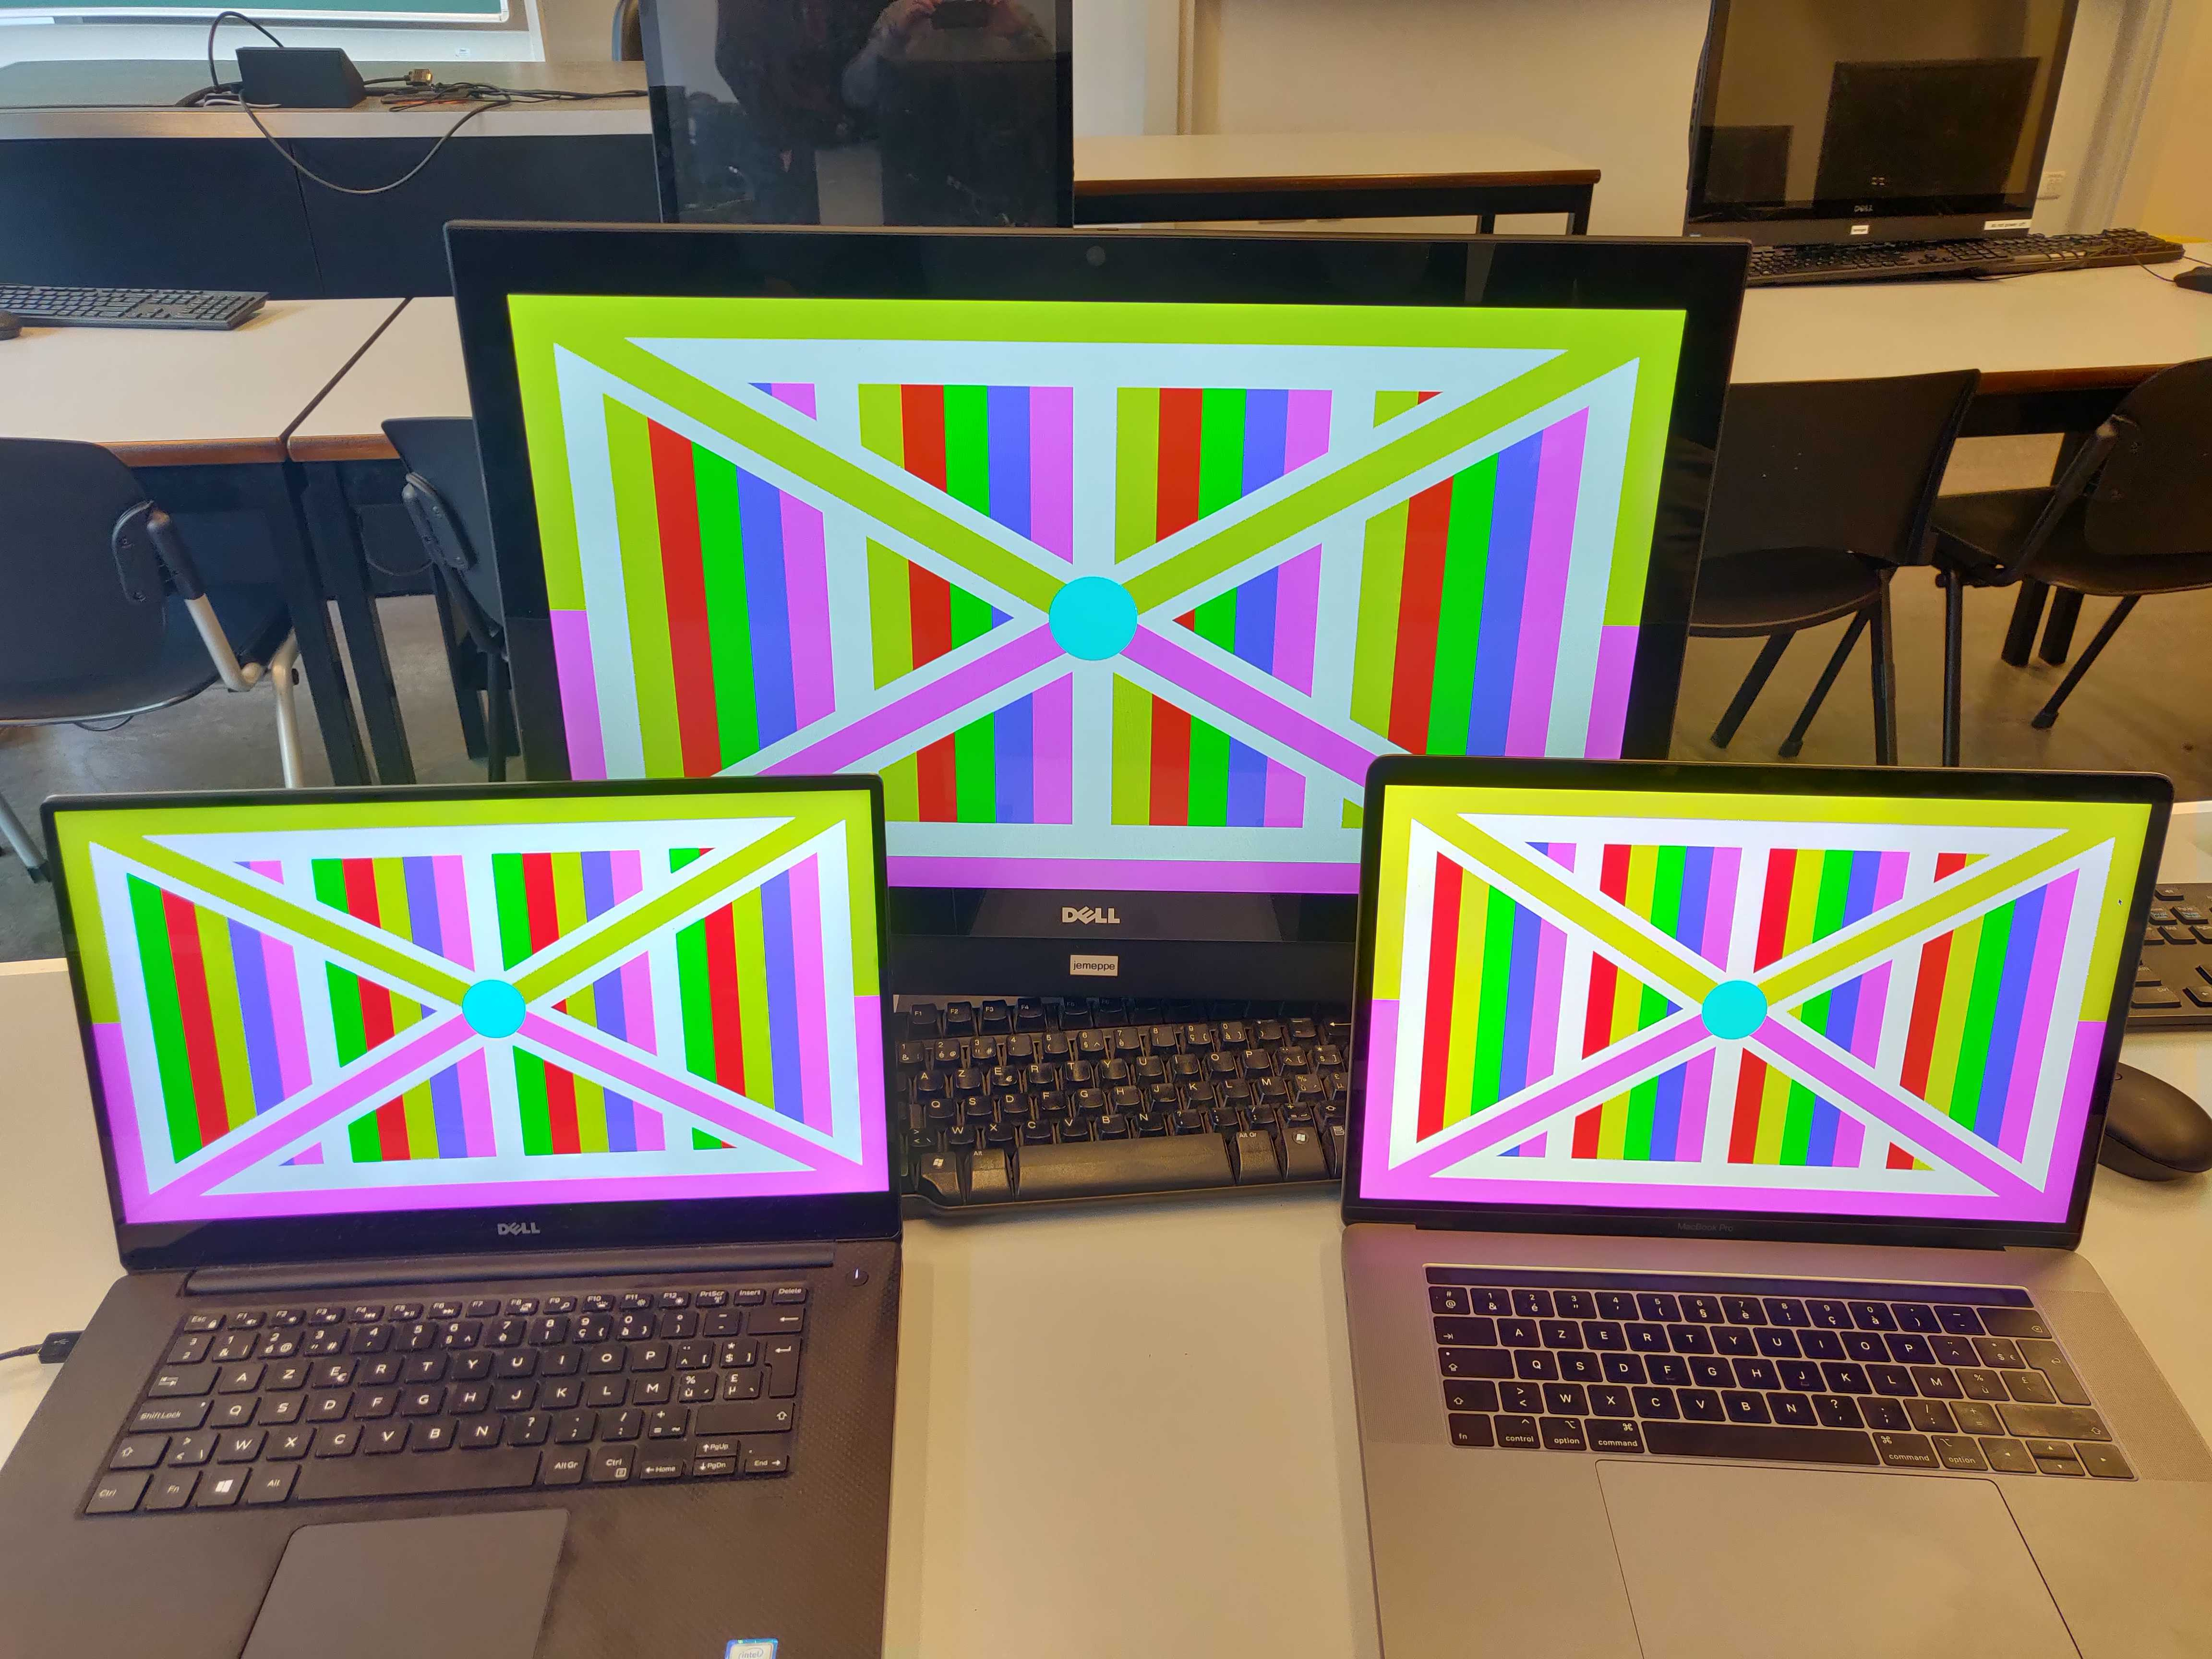
\includegraphics[scale=0.06]{img/opstelling.jpg}
	\caption{Opstelling waarvan een foto wordt genomen.}
	\label{fig:opstelling}
\end{figure}

\paragraph{Hoekdetectie}
Vervolgens zoekt het algoritme naar hoeken, zie bijlage \ref{bijlageA2}. Er wordt gekeken of het scherm gekanteld of recht staat en met deze info het bijpassende hoekdetectie algoritme toegepast. Hierna worden de hoeken gefilterd en zijn de hoeken gedetecteerd. Als er niet genoeg hoeken gevonden zijn, is het geen geldig {\it island}.

\paragraph{Hoekreconstructie}
In bijlage \ref{bijlageA3} en deel \ref{sec:reconstructie}, staat het hoekreconstructie gedeelte gedetailleerder beschreven. Dit wordt uitgevoerd wanneer er niet genoeg hoeken zijn herkend voor een scherm, maar wel genoeg om te reconstrueren. Het gaat de missende hoeken reconstrueren door de lijnen vanuit de reeds gevonden hoeken te volgen.
\paragraph{}
Met alle hoeken en middelpunt op zak is er een scherm gevonden en wordt het geïdentificeerd met behulp van een barcode. Het scherm wordt toegewezen aan een cliënt. Het zoeken gaat verder tot alle cliënts gevonden zijn of alle pixels uit de afbeelding zijn overlopen.

\paragraph{Triangulatie}
Na de analyse wordt het resultaat getoond aan de hand van de Delaunay triangulatie, weergegeven in figuur \ref{fig:triang}. Schermen die niet gedetecteerd werden, worden hierin niet betrokken.
\begin{figure}[H]
	\centering
	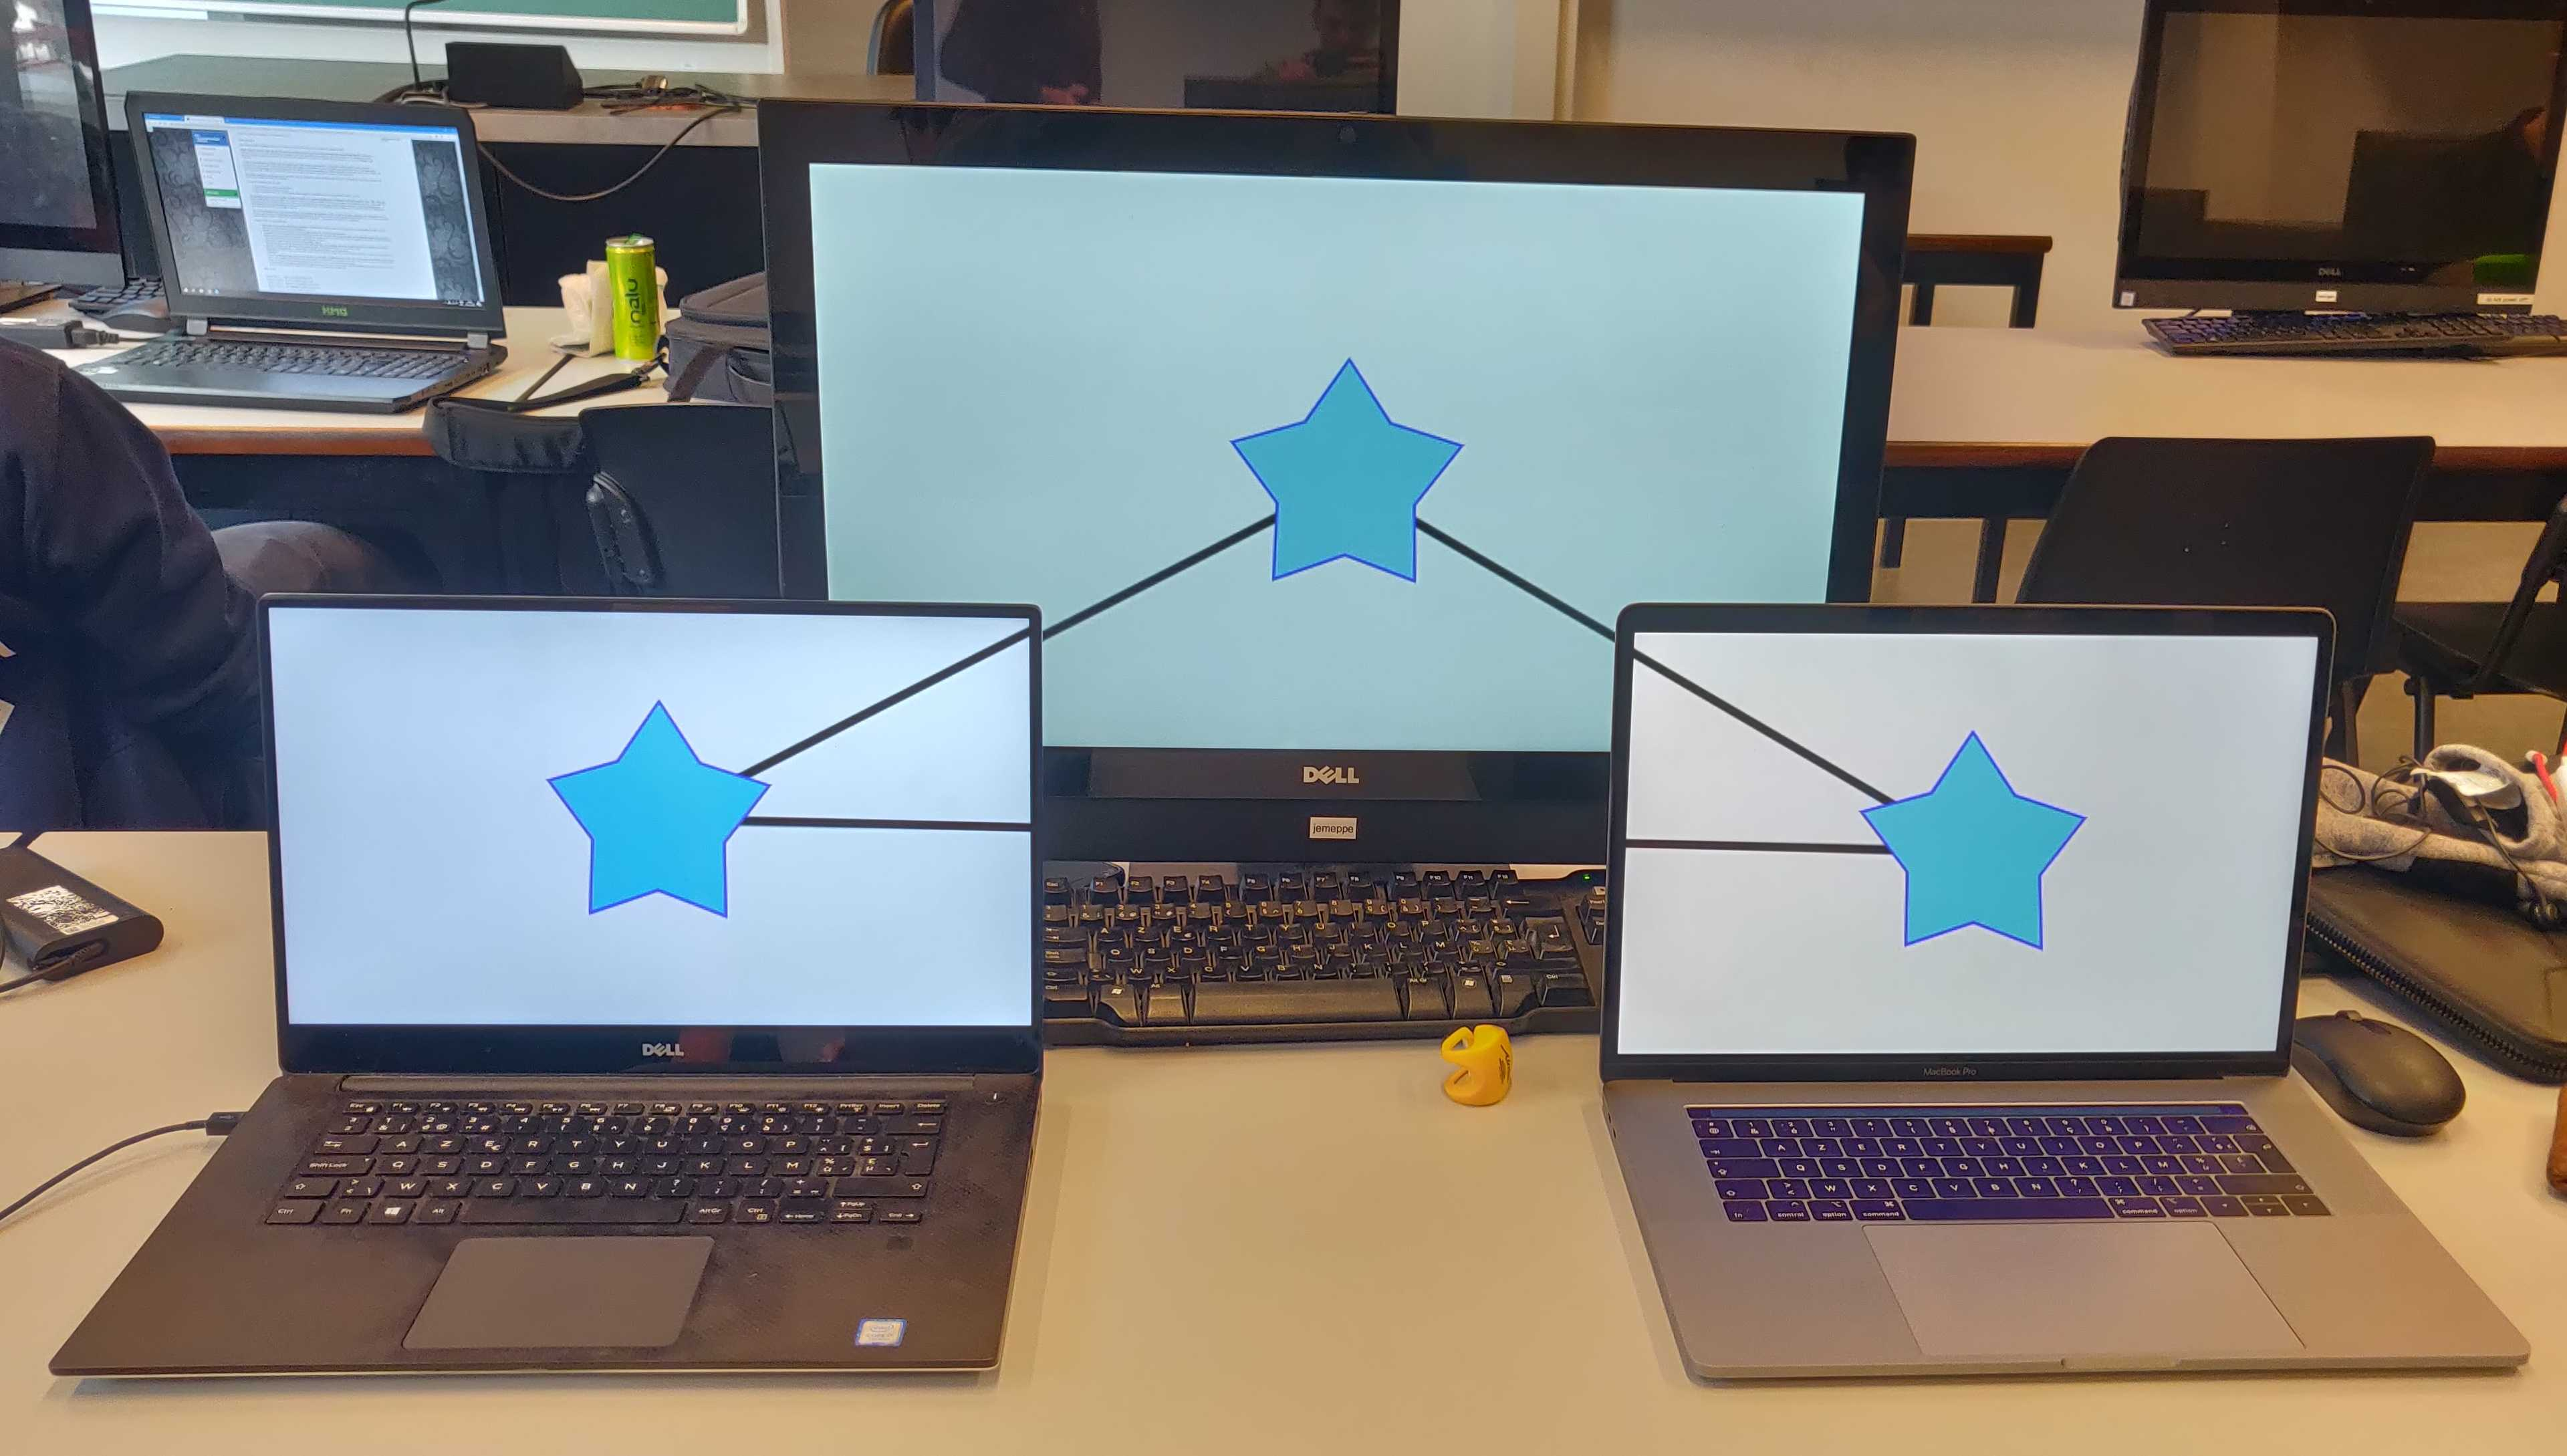
\includegraphics[scale=0.09]{img/triang.jpg}
	\caption{opstelling na detectie van de schermen.}
	\label{fig:triang}
\end{figure}

\paragraph{Afbeelding  weergeven}
Nu kan de master een foto nemen of selecteren uit zijn bestanden om weer te geven op de verbonden toestellen. Voor elk scherm wordt zijn transformatiematrix toegepast op de afbeelding. Het resultaat is te zien op figuur \ref{fig:resultaat}. Hetzelfde kan ook gedaan worden voor video of animatie.
\begin{figure}[H]
	\centering
	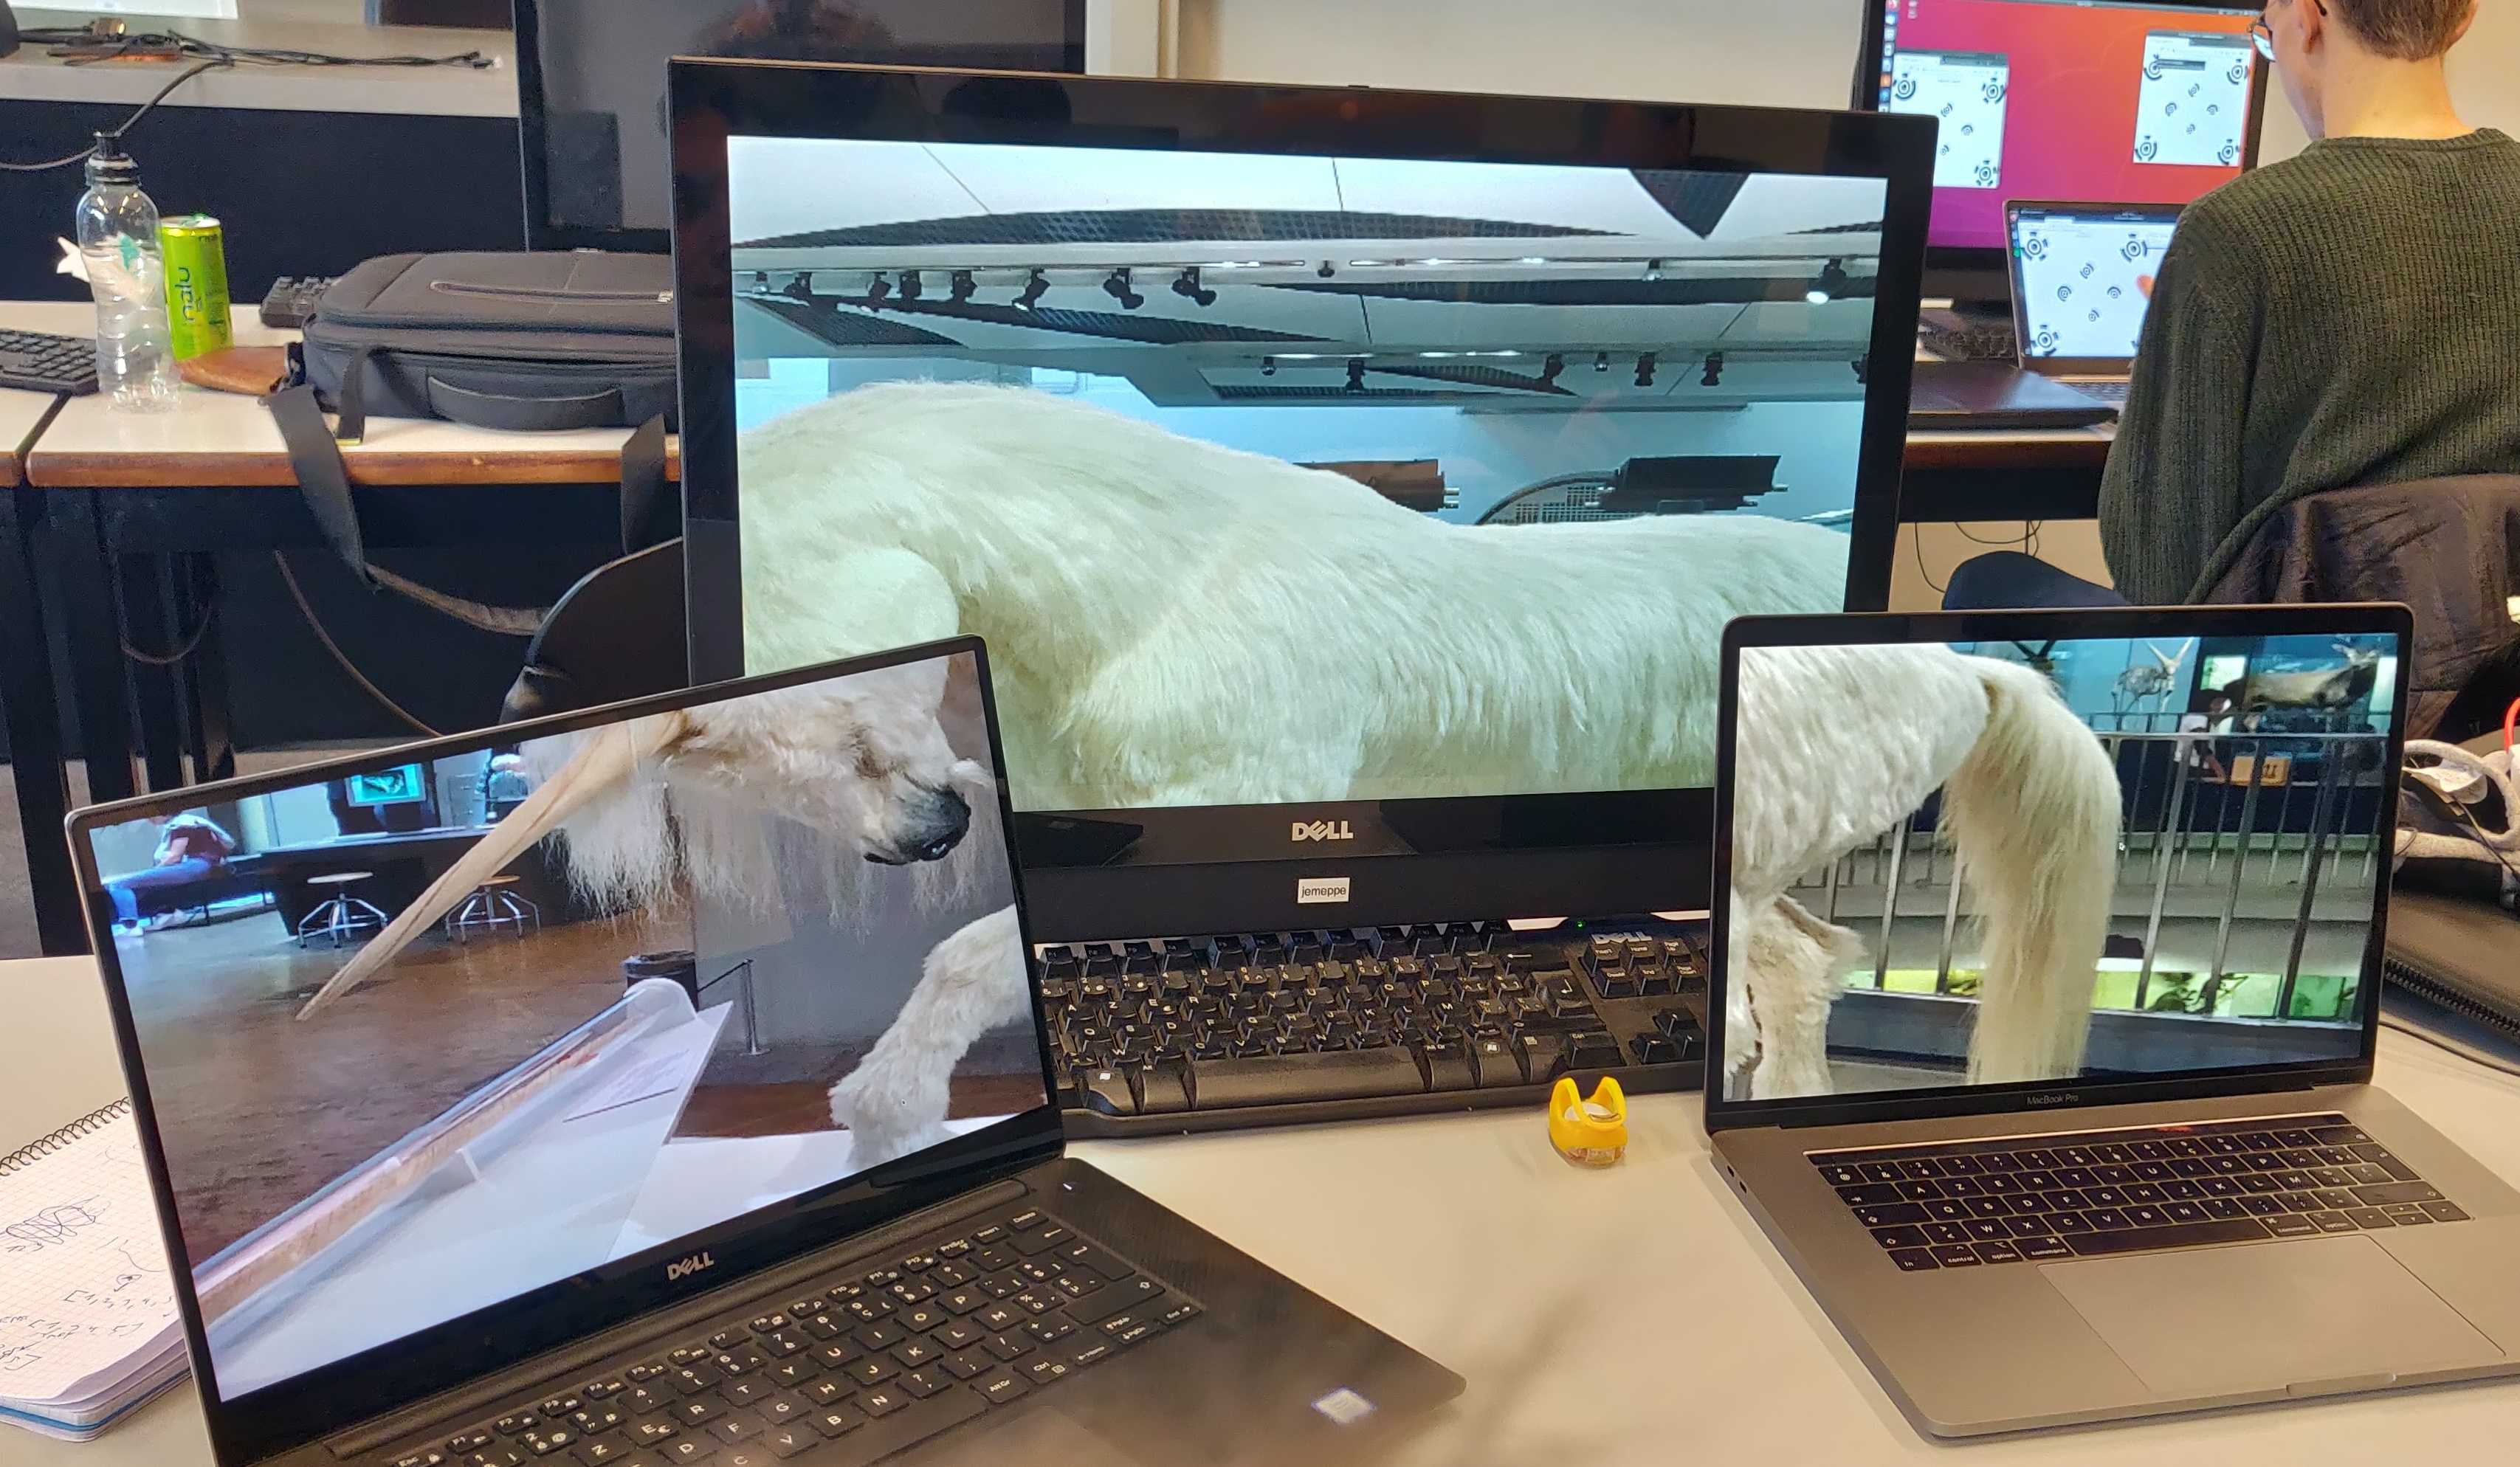
\includegraphics[scale=0.09]{img/resultaat.jpg}
	\caption{De geselecteerde afbeelding weergegeven op de schermen.}
	\label{fig:resultaat}
\end{figure}